To verify the designed and constructed robot as well as its software framework and control methods, a series of field experiments were performed.
The first set of experiments was to test the robot basic movements (such as forward, backward walking and right and lift turn). Some results of these experiments are shown in \ref{robot} (top). The second set was to test the implemented body kinematics. Example results such experiments are given in \ref{robot} (bottom) which shows the robot raising and lowering its body height.
\begin{figure}[H]
	\centering
	\begin{tabular}{ l l }
		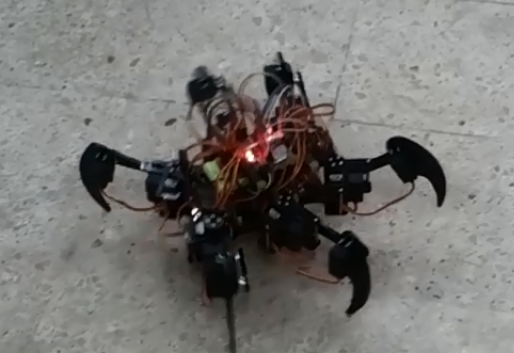
\includegraphics[width =.45\textwidth,height=0.2\textheight]{Fig13_1} & 
        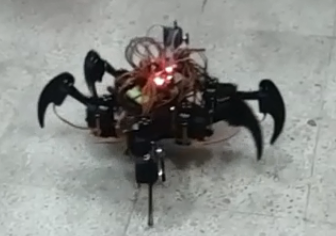
\includegraphics[width =.45\textwidth,height=0.2\textheight]{Fig13_2} \\ 
		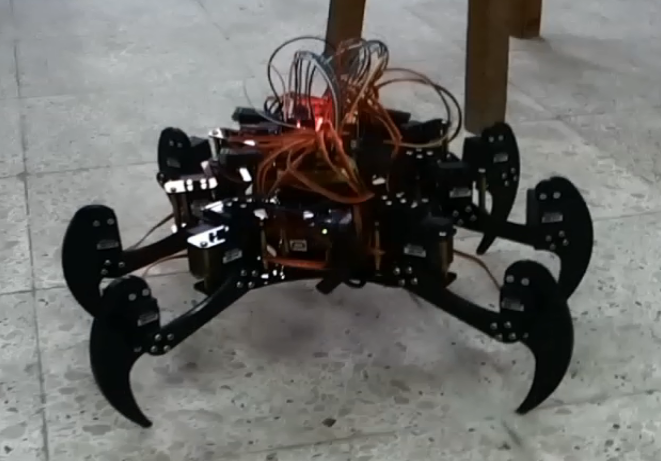
\includegraphics[width =.45\textwidth,height=0.2\textheight]{Fig14_1} & 
        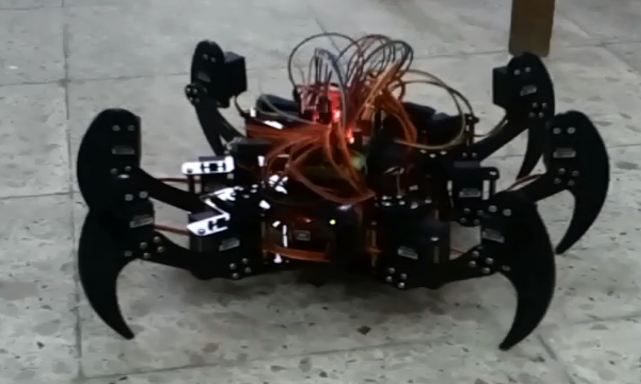
\includegraphics[width =.45\textwidth,height=0.2\textheight]{Fig14_2} \\ 
	\end{tabular}
	\caption{Experiment results: forward and backward move (top) and raising and lowering the body height (bottom).}
	\label{robot}
\end{figure}
\newpage

\section{Simulation}
To help test the design robot and verify software modules and the overall behaviour, the robot is modelled and simulated. The first model for the whole robot is performed in Rviz to test the different ROS nodes and the whole software framework. Rviz is one of ROS tools. It is capable of visualizing many different kinds of information in the same interface. You can load visualization plugins. In the parameters of these plugins you generally define the topic name to which the plugin subscribes, this is fairly straightforward. Rviz configuration file is provided with the sources and started by default in the launch file. Within our ROS-Rviz setup, we simulated the robot movement to test it in different conditions. That made it much easier and faster than apply all the scenarios on the real robot.

In the second simulation, we modelled the robot in MATLAB and employing the Robotics Toolbox. The main purpose of this simulation is to calculate and simulate the kinematics of robot. To create the six-legged walking robot, we started by creating a three-axis robot arm that we used as a leg. Then we implemented a trajectory for the leg that is suitable for walking. Finally, we instantiated six instances of the leg to create the walking robot. The equations given in Sec.4 are programmed first for one leg and tested on successful working, the whole body kinematics were also programmed and tested.
The results were very useful in modifying the walking gaits of the robot which then implemented in the real robot. Figure 10 shows one such simulations in which the same experiment performed on the real robot to test the whole body kinematics for raising and lowering the body height.

\begin{figure}[h]
	\centering
	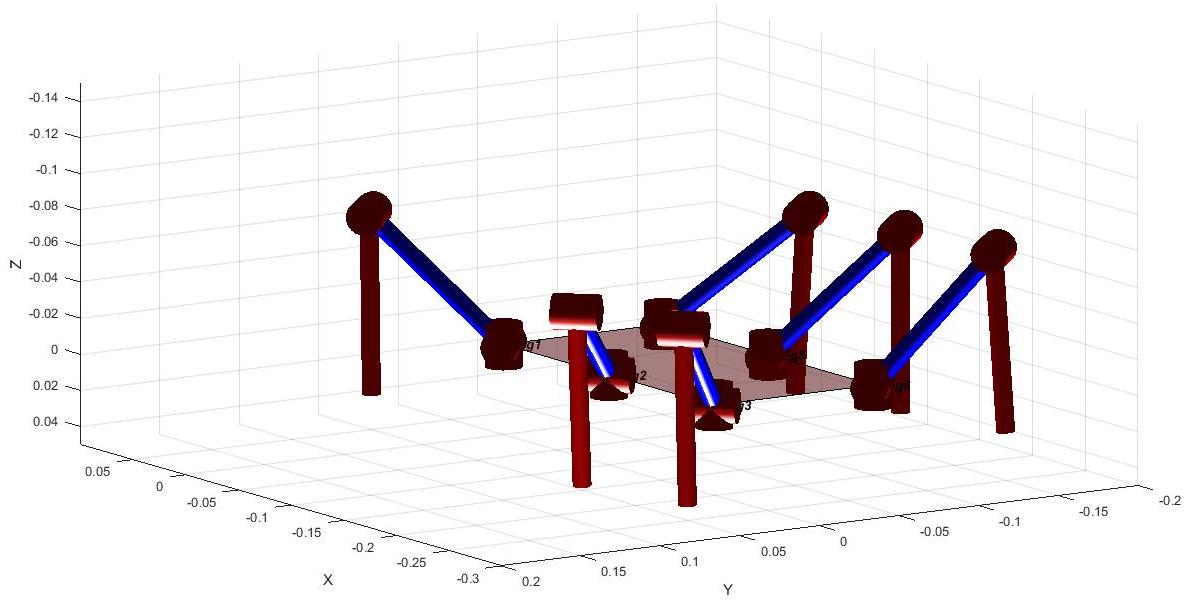
\includegraphics[width =.8\textwidth]{Fig15_1.jpg} 
    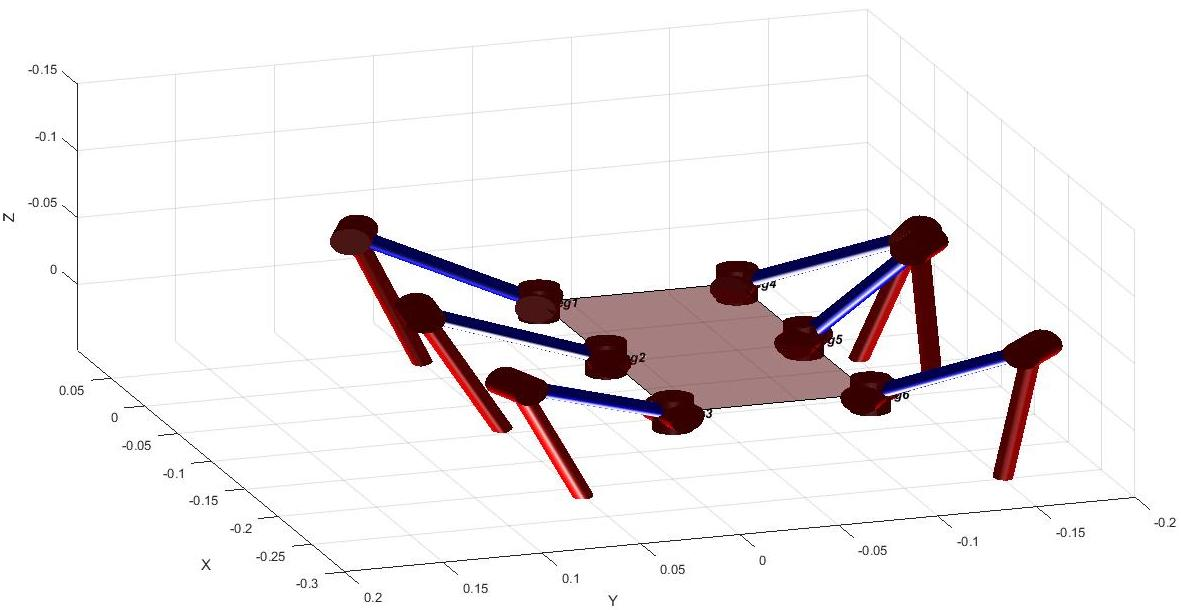
\includegraphics[width =.8\textwidth]{Fig15_2.jpg}
	\caption{ Hexapod robot Simulation.}
	\label{sim}
\end{figure}